\documentclass[a4paper,fleqn]{cas-dc}

\usepackage[numbers,sort&compress]{natbib}
\usepackage{amsmath,amssymb,amsfonts}
\usepackage{booktabs}
\usepackage{multirow}
\usepackage{graphicx}
\usepackage{algorithm}
\usepackage{algpseudocode}
\usepackage{url}
\usepackage{hyperref}
\usepackage{xcolor}
\usepackage{makecell}
\usepackage[section]{placeins}
\raggedbottom

\renewcommand{\topfraction}{0.95}
\renewcommand{\bottomfraction}{0.9}
\renewcommand{\textfraction}{0.08}
\renewcommand{\floatpagefraction}{0.9}
\renewcommand{\dbltopfraction}{0.95}
\renewcommand{\dblfloatpagefraction}{0.9}
\setcounter{topnumber}{5}
\setcounter{bottomnumber}{4}
\setcounter{totalnumber}{8}
\setcounter{dbltopnumber}{2}

\setlength{\textfloatsep}{8pt plus 2pt minus 2pt}
\setlength{\floatsep}{6pt plus 2pt minus 2pt}
\setlength{\intextsep}{8pt plus 2pt minus 2pt}
\setlength{\dbltextfloatsep}{8pt plus 2pt minus 2pt}

\makeatletter
\def\fps@figure{tbp}
\def\fps@table{tbp}
\makeatother

\begin{document}

% -------------------------------------------------
% Front matter
% -------------------------------------------------
\shorttitle{DeepFlow RL for edge-cloud LLM Inference}
\shortauthors{Chen et al.}



\title [mode=title]{DeepFlow RL: Token-Based Speculative Inference for Adaptive Edge-Cloud Collaborative LLM Serving under Weak Network}

% 作者信息
\author[university]{Jiawei Chen}
\ead{202321331009@jmu.edu.cn}

\author[university]{Jian Mao}[orcid=0000-0003-1345-7408]
\cormark[1]
\ead{maojian@jmu.edu.cn}

\author[university]{Xiaowen Huang}
\ead{xwhuang@jmu.edu.cn}

\author[university]{Xiang Liu}
\ead{202321331059@jmu.edu.cn}

\author[university]{Zihao Lin}
\ead{202321331047@jmu.edu.cn}

\author[university]{Yikai Shen}
\ead{202321331028@jmu.edu.cn}

\cortext[1]{Corresponding author.}

\affiliation[university]{
    organization={College of Computer Engineering, Jimei University},
    addressline={No. 185 Yinjiang Road, Jimei District},
    city={Xiamen},
    postcode={361021},
    state={Fujian},
    country={China}
}

% -------------------------------------------------
% Abstract / Keywords
% -------------------------------------------------
\begin{abstract}
\noindent
Edge-cloud collaboration is an important way to relieve the computation and memory pressure of deploying large language models (LLMs) on edge devices. However, the communication costs associated with collaborative inference data may outweigh the benefits of cloud execution under weak network conditions. To address this issue, DeepFlow with Reinforcement Learning (DeepFlow RL) is proposed as a token-based speculative inference framework for adaptive edge-cloud collaborative LLM serving. DeepFlow RL reformulates speculative inference as a semantic-level collaboration mechanism between the edge and the cloud. It then replaces intermediate activation transmission with lightweight token-ID transfer to reduce cross-device communication overhead. An elastic micro-batch mechanism is further introduced to alleviate stop-and-wait overhead under high-latency network settings. To adapt the system to different network, workload, and resource conditions, a PPO-based policy is introduced in DeepFlow RL to jointly select the protocol mode, speculative depth, and micro-batch granularity. A unified resource-aware analytical simulator is developed to support policy training and evaluation under consistent computation, communication, verification, memory-feasibility, and system-constraint assumptions. Experiments on the unified backend show that, under a representative weak network setting, DeepFlow-RL achieves an 11.01$\times$ throughput improvement over the best feasible local baseline and about a 3.75$\times$ improvement over a conventional activation-transfer-based collaborative baseline. Experiments under diverse network and workload settings further show that token-based speculative collaboration can deliver stable and interpretable adaptive decisions, and offers a promising design direction for weak network edge-cloud collaborative LLM serving by balancing communication efficiency and runtime adaptability.
\end{abstract}

\begin{keywords}
Edge-Cloud Collaborative Inference \sep Large Language Models \sep Speculative Inference \sep Token Transmission \sep Adaptive Scheduling \sep Weak Network Serving
\end{keywords}

\maketitle

% -------------------------------------------------
% Main sections
% -------------------------------------------------
\section{Introduction}

\begin{figure}
    \centering
    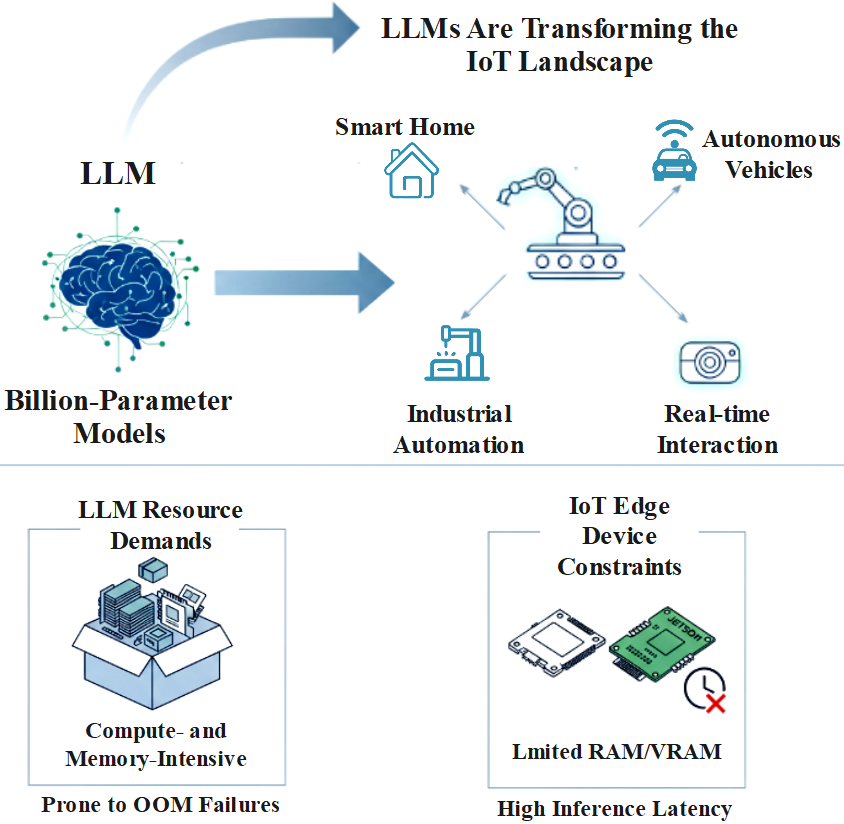
\includegraphics[width=\linewidth]{fig1_my_introduction_image_1.png}
    \caption{Deploying large language models on edge devices faces significant computation and memory constraints.}
    \label{fig:1}
\end{figure}

The rapid development of large language models (LLMs) is pushing intelligent capabilities beyond the cloud and toward the edge, enabling new application scenarios such as smart terminals, industrial control, robotic collaboration, and real-time human-computer interaction~\cite{chen2026network_edge_inference}. However, edge devices are usually constrained by limited compute capability, memory capacity, and energy budgets, and are therefore not well suited for real-time inference with models containing billions or even tens of billions of parameters. This challenge is further aggravated by the high memory demand of current LLM serving, where the growth of request-dependent KV cache can quickly become a primary system bottleneck \cite{kwon2023pagedattention,zhang2025jenga}. On such resource-constrained platforms, purely local execution often suffers from high inference latency and may even trigger out-of-memory failures, making it difficult to satisfy practical deployment requirements for low latency and high availability.

However, these deployment settings usually do not enjoy the stable and high-bandwidth interconnects available inside data centers. In practical edge intelligence deployments, the connection between end devices and edge/cloud servers is often unstable and far less capable than the high-bandwidth interconnects available inside data centers. Under weak network conditions, cross-device communication can easily evolve from a secondary overhead into the dominant system bottleneck, so the effectiveness of collaborative inference depends not only on how computation is distributed across devices, but also on whether the communication cost introduced by collaboration remains affordable.

To alleviate local resource bottlenecks under such constraints, edge-cloud collaborative inference has been widely regarded as a promising solution in both classical split computing and more recent LLM inference systems \cite{kang2017neurosurgeon,patel2024splitwise,mudvari2024splitllm,chen2025adaptivelayersplitting}. Splitting model execution between the edge and the cloud, this approach aims to balance computation placement and resource utilization across devices while minimizing the communication overhead of cross-device collaboration. Conventional collaborative inference usually relies on transmitting intermediate-layer outputs or runtime states across the device boundary. Although such designs may be effective under high-bandwidth interconnects, they are fundamentally limited by bandwidth-constrained cross-device transmission in wide-area weak network settings, where the latency and payload overhead of communication can quickly exceed the benefit brought by cloud execution \cite{kang2017neurosurgeon,patel2024splitwise,mudvari2024splitllm}. Therefore, in weak network edge-cloud inference, the key question is not only \emph{where to partition} the model, but also \emph{what to transmit} across devices.

Motivated by this observation, we propose DeepFlow based on reinforcement learning (DeepFlow RL), a token-based speculative inference framework for adaptive edge-cloud collaborative LLM serving. DeepFlow RL is a token-based speculative inference framework. Through edge-side drafting and cloud-side verification, it replaces cross-device transmission of intermediate activations with lightweight token IDs, thereby reducing communication overhead under weak network conditions. In addition, the system introduces an elastic micro-batch mechanism to mitigate serial waiting overhead under high-latency settings. On top of this, we build a unified resource-aware modeling and policy learning framework that jointly decides the protocol mode, speculative depth, and micro-batch granularity. To address the variation in optimal actions caused by changing network states, workloads, and resource conditions, we employ a PPO-based controller to learn the mapping from system states to actions, enabling adaptive scheduling for runtime scenarios \cite{schulman2017ppo,qin2026twostageppo,fu2024efficient_llm_scheduling}.

The main contributions of this paper are summarized as follows:
\begin{itemize}
    \item By transforming speculative inference from a single-node decoding acceleration technique into a semantic-level collaboration mechanism for weak network edge-cloud inference, and replacing conventional intermediate-state transmission with lightweight token-ID payloads, the proposed design significantly reduces communication overhead under weak network conditions.

    \item By formulating protocol mode, speculative depth, and micro-batch granularity as a joint runtime decision problem and using PPO to learn the mapping from system scenarios to actions, we enable adaptive scheduling under dynamic network and workload conditions.
    
    \item A unified resource-aware modeling and execution backend that jointly characterizes edge-side drafting, network communication, cloud-side verification, memory feasibility, and system constraints is developed to support the training, execution, and performance evaluation of different collaborative strategies under consistent system and modeling assumptions.

    \item Experimental results show that DeepFlow RL outperforms other representative methods under representative weak-network and diverse workload settings. Even when faced with changes in network and workload conditions, DeepFlow RL continues to generate stable and interpretable adaptive decisions.
\end{itemize}

\section{Related Works}
In this section, the related work on edge-cloud collaborative inference, speculative decoding and token-based collaboration, and memory-aware serving, and scheduling is analyzed.

\subsection{Edge-cloud Collaborative Inference}
Edge--cloud collaborative inference predates the emergence of large language models. Earlier studies had already explored how to partition neural network execution across end devices, edge nodes, and the cloud. Teerapittayanon et al.\ proposed a distributed DNN execution framework, Jeong et al.\ systematically studied cross-device partition point selection in Neurosurgeon, and other researchers further advanced split computing from the perspectives of latency optimization, energy constraints, runtime scheduling, and heterogeneous deployment, respectively \cite{teerapittayanon2017distributed_dnn,kang2017neurosurgeon,li2020edge_ai,eshratifar2021jointdnn,laskaridis2020spinn,huang2022aodnn}. Together, these studies show that the benefit of distributed inference depends on the balance among computation placement, communication cost, and device capability.

As LLM inference has become a major systems topic, related work has extended these ideas to large-model settings. Patel et al.\ pointed out in Splitwise that the prefill and decode stages of generative LLMs differ substantially in computation intensity, throughput characteristics, and state migration cost, making stage-aware cross-device organization particularly important \cite{patel2024splitwise}. Mudvari et al.\ studied server--client collaborative LLM inference in SplitLLM and used dynamic programming to optimize partitioning under communication cost and service constraints \cite{mudvari2024splitllm}. Chen et al.\ further considered dynamic partitioning in wireless edge environments \cite{chen2025adaptivelayersplitting}; Zhang et al.\ and Jin et al.\ expanded the system design space of LLM inference from the perspectives of edge sharding collaboration and edge-cloud collaborative serving, respectively \cite{zhang2025edgeshard,jin2024cecollm}. In addition, recent surveys suggest that collaboration between small edge models and large cloud models has evolved from simple layer-wise partitioning to a broader spectrum including task collaboration, model collaboration, and hybrid execution \cite{li2025edgecloudsurvey,cai2026edge_llm_survey}.

Despite this progress, most existing edge-cloud collaborative methods still assume that moving intermediate activations or runtime states across devices is reasonable, and therefore mainly focus on \emph{how to partition the model} and \emph{how to place computation} \cite{kang2017neurosurgeon,patel2024splitwise,mudvari2024splitllm,chen2025adaptivelayersplitting,zhang2025edgeshard,jin2024cecollm}. In contrast, our work does not continue to optimize within the conventional activation/state transfer path. Instead, it revisits the transmission primitive itself under weak network conditions by replacing high-dimensional intermediate-state transfer with lightweight token-ID transfer, thereby shifting edge-cloud collaboration from activation-level offloading to semantic-level collaboration.

\subsection{Speculative Decoding and Token-Based Collaboration}

Speculative decoding was originally proposed as a \emph{single-node decoding acceleration} method. Its key idea is to let a lightweight draft model generate candidate tokens and then let a stronger target model verify them in parallel, thereby improving inference throughput while preserving the output distribution \cite{stern2018blockwise,leviathan2023speculative}. Building on this idea, recent studies have mainly advanced along three directions. One line of work improves candidate generation structures \cite{cai2024medusa,ankner2024hydra}. Another line extends the organization of candidate verification, including tree-based verification, speculative streaming, and cascaded speculation~\cite{miao2024specinfer,bhendawade2024speculativestreaming,narasimhan2025fastercascades}. A third line further investigates the relationship between speculative gain, feature modeling, lookahead inference, and broader serving-system implications~\cite{li2024eagle,fu2026scaling,kumar2026speculative,miao2025efficient_llm_serving_survey}.

Overall, these studies treat speculative decoding as a means to improve decoding efficiency in local or tightly coupled serving frameworks. Their main focus is how to obtain higher speculative gain, how to improve candidate generation quality, and how to improve parallel verification efficiency on a single machine or under homogeneous hardware settings \cite{leviathan2023speculative,cai2024medusa,miao2024specinfer,li2024eagle,fu2026scaling,kumar2026speculative}. In contrast, our work does not view speculative decoding merely as a local acceleration technique. Instead, we reorganize it as a cross-device protocol for weak network edge-cloud collaboration: the draft--verify structure serves not only as an algorithmic mechanism for parallel token verification, but also as a communication mechanism that replaces activation transfer with token-ID transfer. Therefore, our main concern is no longer how to further improve single-node speculative gain, but how to use the speculative structure to change the transmission primitive in edge-cloud collaboration.

\subsection{Memory-Aware Serving, Scheduling, and Simulation}

Beyond computation itself, the system performance of LLM serving is also strongly affected by KV cache, runtime memory organization, request scheduling, and multi-stage execution patterns. In memory management, Kwon et al.\ showed in vLLM/PagedAttention that inefficient KV-cache management can directly limit feasible batch size and system throughput \cite{kwon2023pagedattention}. Zhang et al.\ further pointed out that, under heterogeneous architectures, GPU capacity and KV-cache placement/eviction strategies become core constraints during serving \cite{zhang2025jenga}. Building on this line of work, Zhu et al.\ studied redundant memory access caused by long shared prompts~\cite{zhu2024relayattention}, while Liu, Pan, Qin, and others advanced cache and memory system design from the perspectives of KV-cache compression and streaming, prefix caching, and KV-centric disaggregation~\cite{liu2024cachegen,pan2025marconi,qin2025mooncake}. Related studies further show that prefix reuse, cache hits, and query scheduling continue to affect the performance boundary of real serving systems \cite{wang2025kvcachewild,dexter2026llm}.

In runtime scheduling, prior work has also revealed the importance of stage heterogeneity and request organization from different angles. Zheng et al.\ emphasized in SGLang the coupling between structured multi-call programs and cache-aware execution \cite{zheng2024sglang}. Zhong et al.\ showed in DistServe that prefill and decode have different resource demands and latency objectives, and co-locating them can introduce substantial stage interference \cite{zhong2024distserve}. In addition, recent studies have optimized the runtime organization of LLM and MLLM serving from the perspectives of edge--cloud continuum task scheduling, learning-based request scheduling, and goodput-oriented serving optimization~\cite{zhang2026eco_efficient_mllm_scheduling,fu2024efficient_llm_scheduling,hu2025bestserve}. More broadly, stage heterogeneity, stage overlap, and waiting cost have also been recognized as important issues in LLM serving systems, especially in phase-splitting and prefill--decode disaggregation settings~\cite{patel2024splitwise,zhong2024distserve}.

Finally, our work is also related to analytical modeling and simulation-driven evaluation. The Roofline model proposed by Williams et al.\ provides a classical tool for approximating execution performance using compute and bandwidth upper bounds \cite{williams2009roofline}. More recent simulation frameworks for LLM serving, such as Vidur by Agrawal et al., LLMServingSim 2.0 by Cho et al., and Phantora by Qin et al., have advanced the design of runtime-aware simulators from the perspectives of serving simulation, heterogeneous infrastructure modeling, and GPU-cluster performance estimation~\cite{agrawal2024vidur,cho2025llmservingsim2,qin2026phantora}.

Compared with the above studies, this paper focuses on a more specific systems problem: in weak network edge-cloud collaborative inference, how to unify token-based speculative collaboration, memory-aware feasibility, and adaptive control within the same resource-aware framework.

\section{Background and Motivation}

This section analyzes the communication bottleneck of collaborative inference based on activation transfer under weak network conditions, and explains the motivation for DeepFlow-RL in terms of token based speculative collaboration and adaptive scheduling.

\subsection{Communication Wall in Activation-Based edge-cloud Inference}

Most existing edge-cloud collaborative inference systems still essentially follow the paradigm of \emph{activation-level offloading}, where intermediate activations or related runtime states are transmitted across the device boundary \cite{teerapittayanon2017distributed_dnn,kang2017neurosurgeon,li2020edge_ai,eshratifar2021jointdnn,laskaridis2020spinn,huang2022aodnn,patel2024splitwise,mudvari2024splitllm,chen2025adaptivelayersplitting,zhang2025edgeshard,jin2024cecollm}. This design path is reasonable to some extent for traditional DNNs and higher-bandwidth settings, because end-to-end benefits can still be obtained through partition point selection, execution-path organization, or stage partitioning \cite{kang2017neurosurgeon,li2020edge_ai,patel2024splitwise,mudvari2024splitllm}. However, under wide-area weak network conditions, this design exposes a more fundamental issue: the cost of cross-device state migration may quickly exceed the benefit of local computation, turning collaborative inference from a computation-benefit problem into a communication-constrained problem.

\begin{figure}
    \centering
    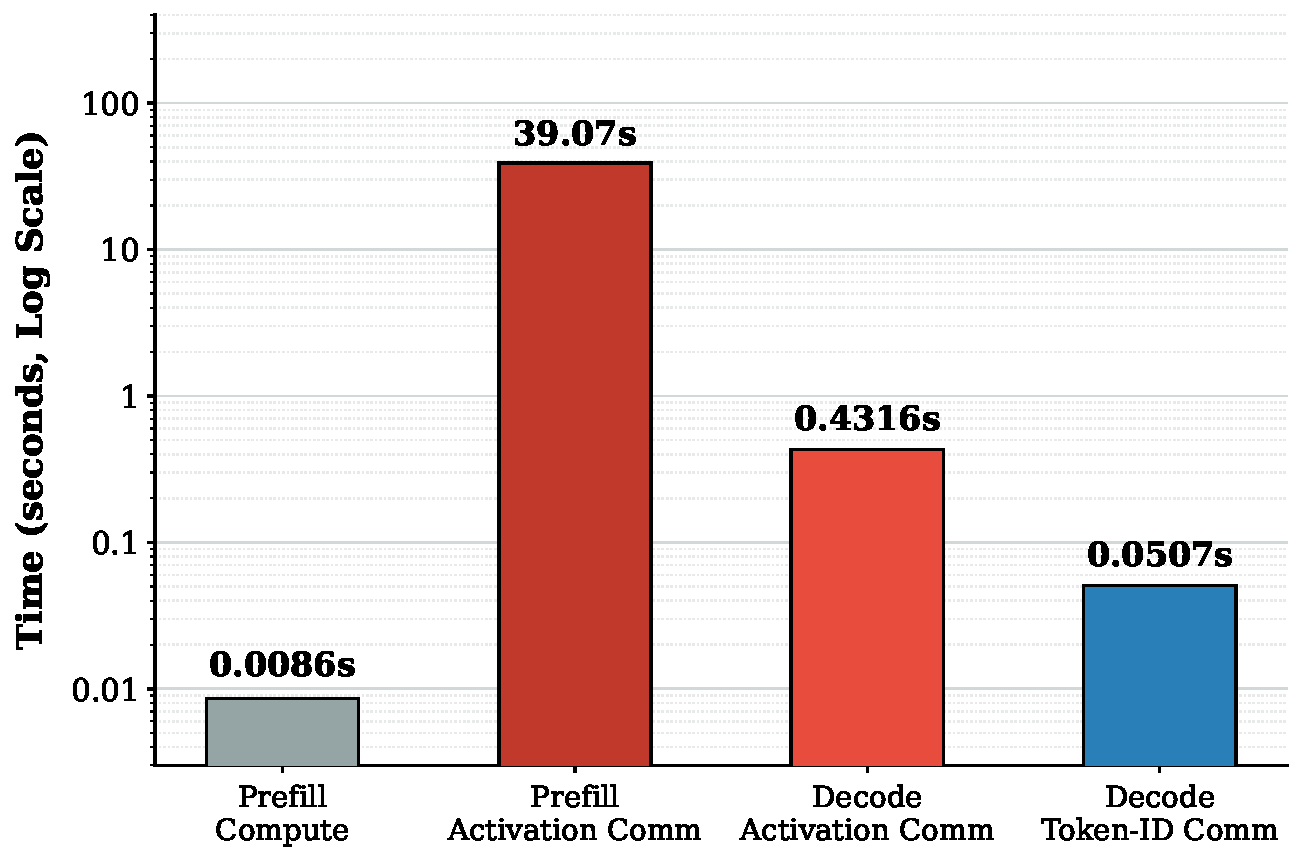
\includegraphics[width=0.96\columnwidth]{fig2_activation_vs_tokenid_cost.pdf}
    \caption{Communication cost under a representative weak network setting.}
    \label{fig:2}
\end{figure}

To quantify this issue, we examine the cost of activation transfer under a representative weak network setting with 1 Mbps bandwidth and 50 ms one-way latency. As shown in Fig.~\ref{fig:2}, for the prefill stage of Llama-2-7B with a prompt length of 512, local computation on the edge takes only 8.56 ms, while transmitting about 4 MB of intermediate activations to the cloud takes as long as 39.07 s. This result suggests that, under weak network conditions, the activation transfer cost in the prefill stage far exceeds the local computation cost, and thus traditional collaborative inference becomes dominated by communication latency. This implies that simply choosing a better partition point is not enough; as long as the transmitted object remains a high-dimensional activation tensor, collaborative inference itself may lose its system-level value.

\subsection{From Activation Transfer to Token-Based Speculative Collaboration}

Motivated by the above observation, we argue that the main challenge in weak network edge-cloud collaborative inference is not how to further refine the partition boundary, but how to redesign the cross-device transmission primitive. To this end, we redefine speculative inference as a semantic-level collaboration protocol for edge-cloud inference. In this design, the edge uses a lightweight draft model to generate candidate tokens and transmits only compact token IDs across devices, while the cloud uses the target model for parallel verification and correction. As a result, speculative inference in our framework is no longer only a local decoding accelerator, but is repurposed as a cross-device semantic-level transmission mechanism.

\begin{figure}
    \centering
    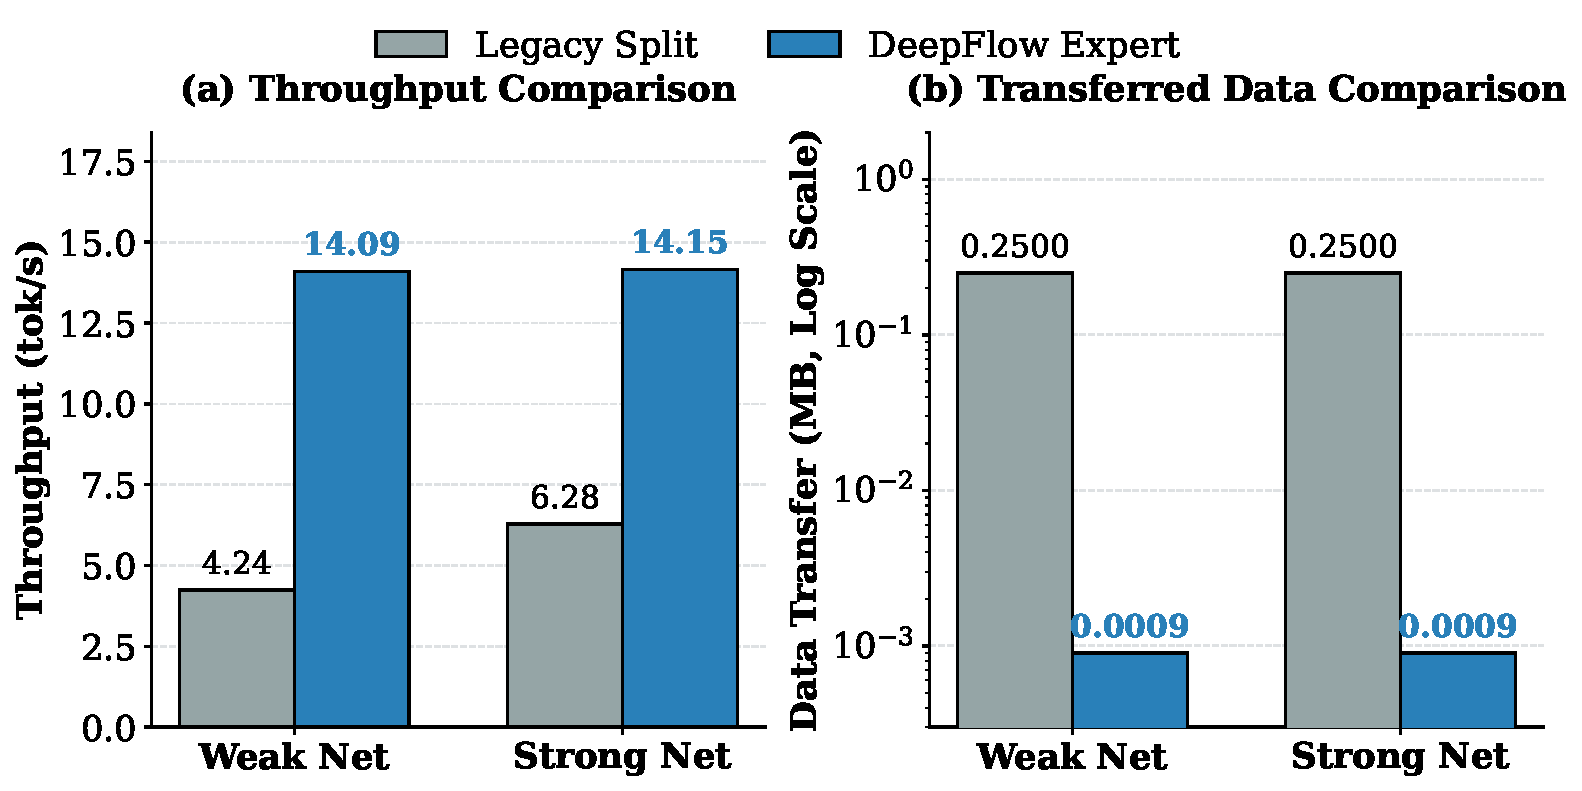
\includegraphics[width=0.96\columnwidth]{fig3_legacy_vs_deepflow.pdf}
    \caption{Comparison between conventional partitioning and token-based DeepFlow under weak and strong network conditions.}
    \label{fig:3}
\end{figure}

Preliminary mechanism-oriented experiments under a fixed example action configuration validate the direct benefit of this design. As shown in Fig.~\ref{fig:2}, under the same weak network condition, when the speculative decoding step is set to $K=5$, activation transfer requires about 0.4316 s of communication time, whereas token-ID transfer requires only 0.0507 s, yielding about an 8.5$\times$ communication-side gain. Furthermore, as shown in Fig.~\ref{fig:3}, under the same experimental setting, the conventional legacy split strategy achieves a throughput of 4.24 tok/s, while the DeepFlow expert strategy reaches 14.09 tok/s, corresponding to about a 3.33$\times$ throughput improvement. At the same time, the amount of cross-device transferred data is reduced from 0.2500 MB to 0.0009 MB. These preliminary results suggest that token-ID transfer is not merely a simple compression trick, but a key mechanism that shifts edge-cloud collaboration from activation-level offloading to semantic-level collaboration. It changes the transmission primitive on which the system relies under weak network conditions, rather than only improving one local cost term.

\subsection{Granularity Trade-offs and the Motivation for Adaptive Policies}

\begin{figure}
    \centering
    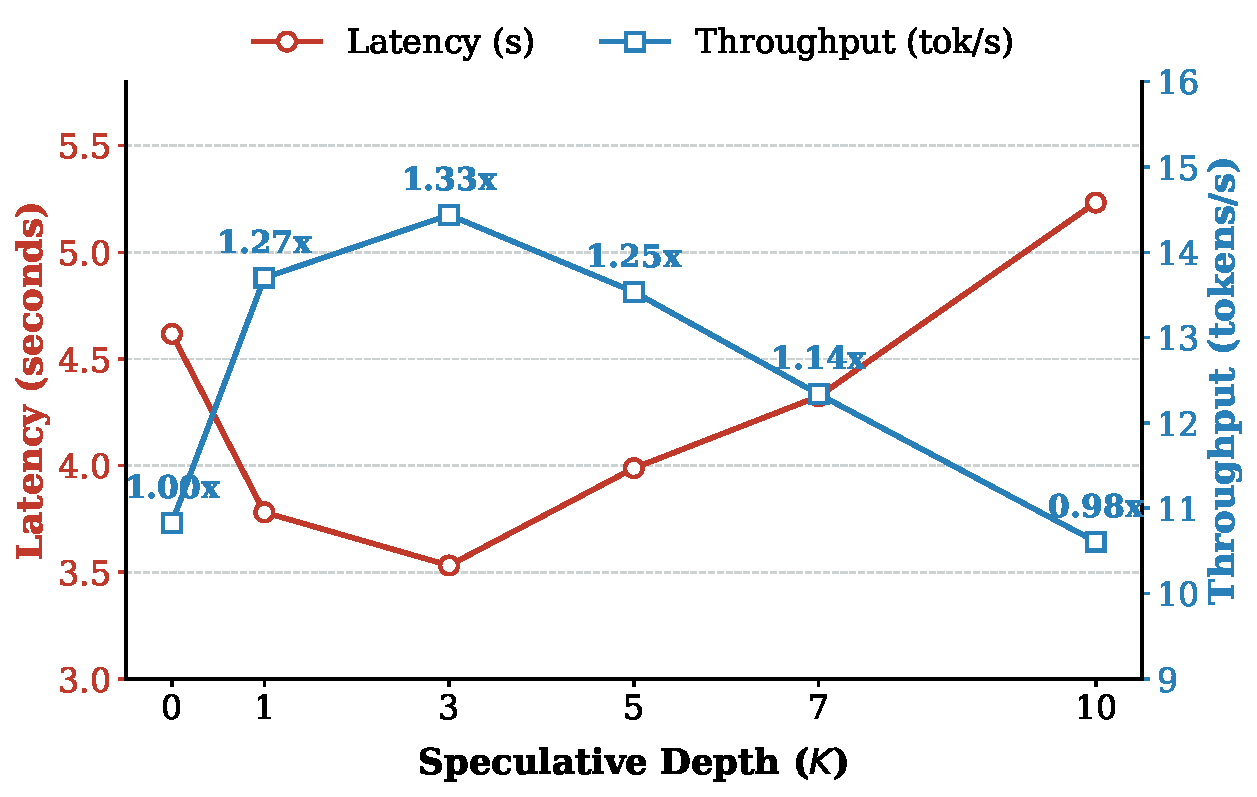
\includegraphics[width=0.96\columnwidth]{fig4_k_sweep.pdf}
    \caption{Throughput--latency trade-off under different speculative depths $K$.}
    \label{fig:4}
\end{figure}

Although token-ID transfer substantially alleviates the communication bottleneck, system efficiency remains highly sensitive to both speculation and pipeline granularity. Fig.~\ref{fig:4} shows the scan results over different speculative depths $K$ under the unified backend. Under the setting of 1 Mbps bandwidth, 50 ms RTT, and a prompt length of 512, the throughput exhibits clear variation across different $K$ values. This suggests that speculative depth has an effective operating range rather than being a monotonically beneficial variable. As $K$ continues to increase, the extra edge-side drafting cost, the enlarged verification length, and the associated resource overhead gradually offset the benefit brought by speculation.

\begin{figure}
    \centering
    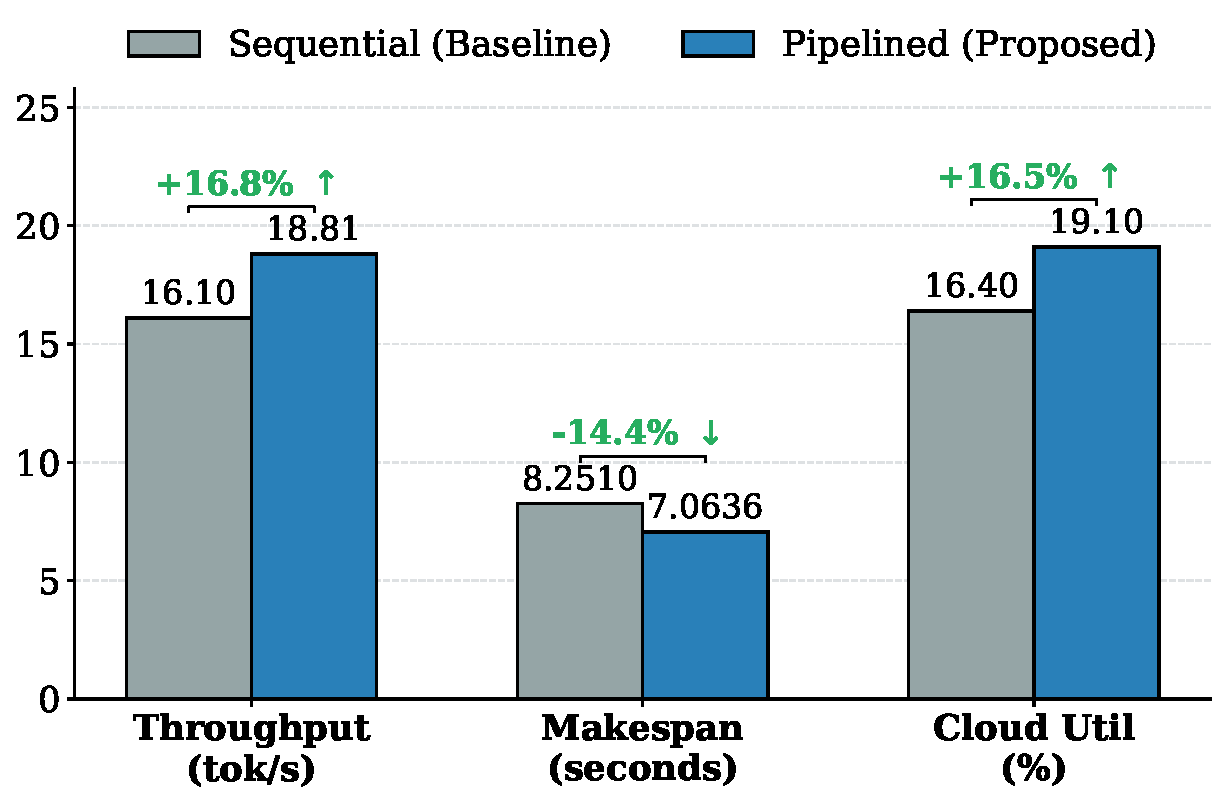
\includegraphics[width=0.96\columnwidth]{fig5_pipeline_vs_sequential.pdf}
    \caption{Effect of micro-batch pipelining. Proper pipelining can improve throughput and cloud utilization while reducing end-to-end makespan.}
    \label{fig:5}
\end{figure}

Fig.~\ref{fig:5} further shows that execution granularity is also important at the pipeline level. In an experiment with batch size 32, $K=5$, and prompt length 512, the system achieves 16.17 tok/s under sequential execution (\textit{micro-batch size}=32). When the task is divided into \textit{micro-batch size}=4 and executed in a pipelined manner, the throughput increases to 18.89 tok/s, corresponding to about a 1.17$\times$ throughput gain. This indicates that an appropriate micro-batch partition can reduce serial idle gaps and improve cloud utilization by overlapping edge-side drafting, network transmission, and cloud verification; however, overly fine granularity may also introduce extra handshake and stop-and-wait overhead.

Taken together, these results suggest that weak network edge-cloud collaborative inference cannot be handled well by a single fixed strategy. Instead, it is a joint decision problem shaped by network conditions, workload characteristics, and system resource states. The transmission primitive should be chosen properly to avoid the activation-transfer bottleneck; speculative depth should balance acceptance gain against drafting and verification cost; and micro-batch size should trade off overlap opportunities against RTT-sensitive stop-and-wait overhead. These factors are jointly constrained by bandwidth, latency, prompt length, and memory feasibility. Therefore, compared with static heuristic configurations, a controller that can adaptively output $(P,K,M)$ according to runtime states is more appropriate. This is also the direct motivation for DeepFlow RL, and a further analysis of the learned action patterns will be presented in Section~7.

\section{System Model and Problem Formulation}

\subsection{System Abstraction}

weak network edge-cloud collaborative inference is abstracted as a graph composed of a node set and a link set:
\begin{equation}
G=(V,E),
\end{equation}
where $V=\{v_e,v_c\}$ denotes the set of compute nodes, with $v_e$ representing the edge device and $v_c$ representing the cloud server, and $E=\{(v_e,v_c)\}$ denotes the wide-area network link connecting the edge and the cloud. This abstraction characterizes the two-end collaborative inference architecture considered in this paper, in which the edge is responsible for drafting or prefix execution, whereas the cloud is responsible for target-model verification and suffix computation.

Let $\mathcal{T}=\{1,2,\dots,T\}$ denote the discrete decision horizon of the system, and let $t\in\mathcal{T}$ denote an individual decision step. At decision step $t$, the current collaborative inference scenario is characterized by the currently available link bandwidth $W_t$, round-trip latency $\tau_t$, and input prompt length $L_t$. Together, these variables describe the runtime context of the system and provide the basis for subsequent scheduling decisions and performance modeling.  

A lightweight draft model is denoted by $\mathcal{M}_d$ and deployed on the edge, while the target model is denoted by $\mathcal{M}_{\mathrm{tar}}$ and deployed on the cloud. Suppose $\mathcal{M}_{\mathrm{tar}}$ has $L$ layers, and the hidden size and intermediate size of layer $l$ are $h_l$ and $i_l$, respectively. For a typical LLaMA-style Transformer layer, the parameter count $N_l$ can be approximated as:
\begin{equation}
N_l = 4h_l^2 + 3h_l i_l + 2h_l,
\end{equation}
where the first two terms correspond to the attention projection module and the MLP module, respectively, and the last term corresponds to the two LayerNorm parameter sets. The memory occupied by the weights of layer $l$ can be written as:
\begin{equation}
M_l^w = \frac{N_l \cdot b_w}{1024^2}\ \text{MB},
\end{equation}
where $b_w$ denotes the number of bytes per parameter.

At decision step $t$, the joint action of the system is defined as:
\begin{equation}
a_t = (P_t, K_t, M_t),
\end{equation}
where:
\begin{itemize}
    \item $P_t \in \{0,1,\dots,L\}$ denotes the protocol mode or the analytical partition point;
    \item $K_t$ denotes the speculative depth;
    \item $M_t$ denotes the micro-batch size.
\end{itemize}

Here, $P_t$ not only denotes the analytical partition point, but also specifies the cross-device transmission primitive: $P_t=0$ indicates that the token-ID collaborative mode of DeepFlow is enabled, whereas $P_t>0$ indicates that the system falls back to an analytical partitioning baseline based on activation transfer.

To compare the system cost of different actions under consistent system and modeling assumptions, we adopt a unified resource-aware analytical/discrete-event simulation backend, which consistently models computation, communication, verification, and memory feasibility, and outputs key metrics including makespan, throughput, timeline, and OOM information. This design follows the general idea of analytical performance modeling, discrete-event execution modeling, and LLM serving simulators, namely approximating system behavior under calibrated abstractions of hardware, memory, and communication, rather than reproducing low-level microarchitectural events cycle by cycle \cite{williams2009roofline,agrawal2024vidur,cho2025llmservingsim2,qin2026phantora}.

\subsection{Token-Based Speculative Collaborative Inference}

A speculative collaborative cycle is composed of three stages: edge-side drafting, protocol-dependent transmission, and cloud-side verification. The verification mechanism follows the general idea of speculative decoding, in which a lightweight draft model first proposes candidate tokens and a stronger target model then verifies them in parallel \cite{leviathan2023speculative,li2024eagle,miao2024specinfer}.

\paragraph{Edge drafting.}
The edge uses $\mathcal{M}_d$ to autoregressively generate $K$ candidate tokens based on the current context. Let the current context length be $L_t$. Then the generation of the $j$-th candidate token can be written as:
\begin{equation}
x_j = \arg\max_{v} p_{\mathcal{M}_d}(v \mid X_t, x_{1:j-1}), \quad j\in\mathcal{J},
\end{equation}
where $\mathcal{J}=\{1,\dots,K\}$ is the set of candidate tokens.

\paragraph{Protocol-dependent transmission.}
If $P = 0$, only the ID sequence of the candidate tokens is transmitted from the edge to the cloud. Since each token ID is encoded as a 32-bit integer, i.e., 4 Bytes per token, the transmission payload for a micro-batch of size $M$ and speculative depth $K$ is given by
\begin{equation}
D_{\text{tok}}(P,M,K) = \frac{4MK}{1024^2}\ \text{MB}.
\end{equation}

If $P > 0$, the system falls back to analytical partitioning based on activation transfer: the edge executes the first $P$ layers of $\mathcal{M}_{\mathrm{tar}}$ and transmits the activation output of layer $P$. The corresponding payload can be written as
\begin{equation}
D_{\text{act}}(P,M,K) = \frac{M(K+1)h_P b_a}{1024^2}\ \text{MB},
\end{equation}
where $b_a$ denotes the number of bytes corresponding to the activation precision (e.g., 2 Bytes for FP16), and the output tensor size is $[M,\,K+1,\,h_P]$. This dual-mode definition allows the system costs of the two transmission primitives to be compared within the same backend \cite{kang2017neurosurgeon,patel2024splitwise,mudvari2024splitllm,chen2025adaptivelayersplitting}.

\paragraph{Cloud verification.}
The cloud uses $\mathcal{M}_{\mathrm{tar}}$ to perform one parallel verification pass on the concatenated context. Let the verification sequence length be
\begin{equation}
S_{\text{ver}} = L_t + K + 1.
\end{equation}
After the cloud completes the verification pass, the actual number of accepted draft tokens is denoted by $N_{\text{acc}}$, and one additional correction token is also generated. Therefore, the effective sequence growth brought by one speculative cycle is
\begin{equation}
Y(K) = 1 + N_{\text{acc}}.
\end{equation}

Let $\alpha$ denote the probability that a draft token is verified and accepted by the target model. Existing empirical studies on speculative decoding suggest that, as the speculative step increases, the acceptance probability tends to decrease because of the accumulated mismatch between the draft distribution and the target distribution \cite{leviathan2023speculative,li2024eagle}. To avoid explicitly evaluating the expectation of $Y(K)$ by replaying draft--target trajectories token by token, a calibrated acceptance-rate curve is adopted. Specifically, the acceptance rate at step $k$, denoted by $\alpha(k)$, is modeled using an exponential decay function. Let the acceptance probability of the $j$-th draft token be $\alpha_j$, then
\begin{equation}
\alpha_j = \alpha_{\text{base}} \gamma^{j-1}, \quad j\in\mathcal{J},
\end{equation}
where $\alpha_{\text{base}} \in (0,1]$ denotes the acceptance rate of the first token, and $\gamma \in (0,1)$ denotes the decay factor. Accordingly, the expected number of effective tokens in one speculative cycle is
\begin{equation}
\mathbb{E}[Y(K)] = 1 + \sum_{j=1}^{K} \alpha_j.
\end{equation}

This acceptance-rate model is not intended to reproduce the exact token-level trajectory of any specific draft-model/target-model pair. Instead, it is used to capture the system-level trend of speculative yield as the speculative depth changes within the unified backend, and to provide consistent input for the subsequent throughput and feasible-region analysis.

\subsection{Latency and Throughput Model}

\subsubsection{Layer latency model}

A hardware-aware Roofline-style approximation is adopted to estimate the latency of a single layer \cite{williams2009roofline}. For the execution of layer $l$ with batch size $B$ and sequence length $S$, the total FLOPs is denoted by $F_l(B,S,\mathrm{mode})$.

The FLOPs of layer $l$ in the prefill stage can be calculated as:
\begin{equation}
F_l^{\mathrm{pre}}(B,S) = 2BS(4h_l^2 + 3h_l i_l) + 4BS^2 h_l.
\end{equation}
The FLOPs of layer $l$ in the decode/verification approximation can be calculated as:
\begin{equation}
F_l^{\mathrm{dec}}(B,S) = 2BS(4h_l^2 + 3h_l i_l) + 4BSh_l.
\end{equation}

Let the available compute capability of device $v$ be $\Pi_v^{\mathrm{ava}}$, and let the available memory bandwidth be $B_v^{\mathrm{ava}}$. The layer latency is approximated by the dominant term between the compute-bound time and the memory-access-bound time:
\begin{equation}
T_l(B,S,v,\mathrm{mode}) = \max \left( \frac{F_l(B,S,\mathrm{mode})}{\Pi_v^{\mathrm{ava}}}, \frac{M_l^w}{B_v^{\mathrm{ava}}} \right).
\end{equation}

This approximation is intended to capture whether a layer is primarily limited by arithmetic throughput or by memory access bandwidth, rather than to suggest that computation and memory access are fully parallel in implementation. In this paper, it is used as a unified upper-bound approximation for relative comparison across different $(P,K,M)$ decisions under the same modeling assumptions \cite{williams2009roofline,agrawal2024vidur}.

\subsubsection{Stage latency}

For one speculative collaborative cycle of a micro-batch, the edge-side drafting time is
\begin{equation}
T_{\mathrm{draft}}(M,K,L_t) = \sum_{j=0}^{K-1} \sum_{l \in \mathcal{M}_d} T_l(M,L_t+j,v_e,\mathrm{dec}),
\end{equation}
where $\mathrm{dec}$ denotes the decoding mode in the layer-level latency model.

If $P > 0$, the edge also needs to execute the prefix layers of $\mathcal{M}_{\mathrm{tar}}$, whose time is
\begin{equation}
T_{\mathrm{prefix}}(P,M,K,L_t) = \sum_{l=1}^{P} T_l(M,S_{\mathrm{ver}},v_e,\mathrm{pre}).
\end{equation}

Therefore, the total edge-side stage time is
\begin{equation}
T_e(P,M,K,L_t) = T_{\mathrm{draft}}(M,K,L_t) + T_{\mathrm{prefix}}(P,M,K,L_t).
\end{equation}

The communication time follows a latency--bandwidth model:
\begin{equation}
T_{\mathrm{comm}}(P,M,K,t) = \tau_t + \frac{D_{\mathrm{comm}}(P,M,K)}{W_t},
\end{equation}
where $D_{\mathrm{comm}}(P,M,K)$ denotes the protocol-dependent communication payload defined above.


The cloud-side verification time is
\begin{equation}
T_{\mathrm{verify}}(P,M,K,L_t) = \sum_{l=P+1}^{L} T_l(M,S_{\mathrm{ver}},v_c,\mathrm{pre}).
\end{equation}

Accordingly, the total system cost of one collaborative cycle is decomposed into three sequential stages: edge-side drafting/prefix execution, cross-device communication, and cloud-side verification \cite{zhong2024distserve}.

\subsubsection{Pipeline makespan and throughput}

Let the total batch size be $B_{\mathrm{tot}}$.Then the number of micro-batches is
\begin{equation}
N = \frac{B_{\mathrm{tot}}}{M}.
\end{equation}

For micro-batch $i$, where $i=1,2,\dots,N$, let the start and end times in the edge, network, and cloud stages be denoted by $(s_e^{(i)}, e_e^{(i)})$, $(s_n^{(i)}, e_n^{(i)})$, and $(s_c^{(i)}, e_c^{(i)})$, respectively. The discrete-event pipeline progression satisfies
\begin{align}
s_e^{(i)} &= e_e^{(i-1)}, \quad e_e^{(i)} = s_e^{(i)} + T_e, \\
s_n^{(i)} &= \max(e_e^{(i)}, e_n^{(i-1)}), \quad e_n^{(i)} = s_n^{(i)} + T_{\mathrm{comm}}, \\
s_c^{(i)} &= \max(e_n^{(i)}, e_c^{(i-1)}), \quad e_c^{(i)} = s_c^{(i)} + T_{\mathrm{verify}}.
\end{align}

The system makespan is defined as the time at which the last micro-batch completes verification on the cloud:
\begin{equation}
T_{\mathrm{make}} = e_c^{(N)}.
\end{equation}

In one speculative cycle, the expected number of effective tokens per sequence is $\mathbb{E}[Y(K)]$, and therefore the total number of effective tokens is
\begin{equation}
N_{\mathrm{eff}} = B_{\mathrm{tot}} \cdot \mathbb{E}[Y(K)].
\end{equation}

The final throughput is defined as
\begin{equation}
\mathcal{T}(P,K,M; s_t) = \frac{B_{\mathrm{tot}} \cdot \mathbb{E}[Y(K)]}{T_{\mathrm{make}}}.
\end{equation}

\subsection{Memory Model and Feasible Region}

Because the edge needs to deploy the draft model and, under some actions, also host the prefix layers of the target model, optimizing only throughput without considering hardware constraints may lead to out-of-memory (OOM) errors. Therefore, the peak memory usage on both the edge and the cloud is explicitly modeled and treated as a feasible-region constraint.

Prior systems have shown that KV-cache growth, cache placement, and memory residency directly determine feasible batch size, latency, and throughput \cite{kwon2023pagedattention,liu2024cachegen,pan2025marconi,qin2025mooncake,zhang2025jenga}. In addition, when long shared prompts or reusable prefixes exist, prompt-side memory traffic, prefix caching, and cache reuse structures can also significantly affect serving efficiency \cite{wang2025kvcachewild,dexter2026llm,zhu2024relayattention}. Therefore, in the current edge-cloud setting, memory is not merely a static capacity upper bound, but also a first-order factor that shapes the feasible action region.

Let the budget ratio coefficient be $\mu \in (0,1)$, and the available memory budgets on the edge and the cloud are:
\begin{equation}
B_e^{\mathrm{mem}} = \mu C_e, 
\end{equation}
and
\begin{equation}
 B_c^{\mathrm{mem}} = \mu C_c,
\end{equation}
where $C_e$ and $C_c$ denote the physical available memory capacities of the edge and cloud devices, respectively.

\paragraph{Edge peak memory.}
The peak memory on the edge consists of framework overhead, draft-model weights, target-model prefix weights, draft KV cache, target-prefix KV cache, and scratch, activation, and communication buffers. The corresponding quantities are defined as follows:
\begin{itemize}
    \item $M_e^{\mathrm{fw}}$: fixed memory overhead on the edge introduced by the inference framework, runtime reservation, and resident system buffers;
    \item $\mathcal{M}_d^w$: draft-model weights;
    \item $\mathcal{M}_{\mathrm{pre}}^w(P)$: target-model prefix weights under partition point $P$;
    \item $m_d^{\mathrm{kv}}(M)$: KV-cache increment of the draft model per generated token for micro-batch size $M$;
    \item $m_{\mathrm{pre}}^{\mathrm{kv}}(M,P)$: per-token KV-cache increment of the target prefix;
    \item $A_d(M)$: maximum activation footprint on the draft side;
    \item $A_{\mathrm{pre}}(M,S_{\mathrm{ver}},P)$: activation footprint on the target-prefix side;
    \item $\rho_b D_{\mathrm{comm}}(P,M,K)$: reserved communication buffer during edge-cloud data transfer.
\end{itemize}

The peak memory in edge is approximated as:
\begin{equation}
\begin{aligned}
M_e^{\mathrm{peak}}
&= M_e^{\mathrm{fw}}
  + \rho_w \left(\mathcal{M}_d^w + \mathcal{M}_{\mathrm{pre}}^w(P)\right) \\
&\quad + \rho_{\mathrm{kv}} \Bigl[
    m_d^{\mathrm{kv}}(M)(L_t + K)
    + m_{\mathrm{pre}}^{\mathrm{kv}}(M,P) S_{\mathrm{ver}}
  \Bigr] \\
&\quad + \rho_a \max \Bigl(
    A_d(M),\,
    A_{\mathrm{pre}}(M,S_{\mathrm{ver}},P), \\
&\qquad\qquad\qquad\quad
    \rho_b D_{\mathrm{comm}}(P,M,K)
  \Bigr).
\end{aligned}
\end{equation}
Here, $\rho_w$, $\rho_{\mathrm{kv}}$, and $\rho_a$ denote the weight reservation factor, KV-cache safety factor, and activation/buffer safety factor, respectively, while $\rho_b$ denotes the communication-buffer scaling factor. 

\paragraph{Cloud peak memory.}
The peak memory on the cloud consists of framework overhead, target-model suffix weights, target-model suffix KV cache, verification workspace, and communication buffer. The corresponding quantities are defined as follows:
\begin{itemize}
    \item $M_c^{\mathrm{fw}}$: fixed memory overhead on the cloud introduced by the inference framework, runtime reservation, and resident system buffers;
    \item $\mathcal{M}_{\mathrm{suf}}^w(P)$: target-model suffix weights under partition point $P$;
    \item $m_{\mathrm{suf}}^{\mathrm{kv}}(M,P)$: per-token KV-cache increment of the target suffix;
    \item $A_{\mathrm{suf}}^\Sigma(M,S_{\mathrm{ver}},P)$: summed suffix activation footprint;
    \item $A_{\mathrm{suf}}^{\max}(M,S_{\mathrm{ver}},P)$: maximum suffix activation footprint.
\end{itemize}

The cloud peak memory is approximated as
\begin{equation}
\begin{aligned}
M_c^{\mathrm{peak}} &= M_c^{\mathrm{fw}} + \rho_w \mathcal{M}_{\mathrm{suf}}^w(P) + \rho_{\mathrm{kv}} m_{\mathrm{suf}}^{\mathrm{kv}}(M,P)S_{\mathrm{ver}} \\
&\quad + \rho_{\mathrm{ws}} \max\left(0.3A_{\mathrm{suf}}^\Sigma, A_{\mathrm{suf}}^{\max}, \rho_b D_{\mathrm{comm}}(P,M,K)\right).
\end{aligned}
\end{equation}
where $\rho_{\mathrm{ws}}$ is the verification-workspace safety factor.

Therefore, an action $a_t=(P_t,K_t,M_t)$ is feasible if and only if
\begin{equation}
M_e^{\mathrm{peak}} \leq B_e^{\mathrm{mem}}
\quad \text{and} \quad
M_c^{\mathrm{peak}} \leq B_c^{\mathrm{mem}}.
\end{equation}
Otherwise, the action is marked as infeasible, and the OOM location is recorded as \texttt{edge}, \texttt{cloud}, or \texttt{both}, depending on which side violates the memory constraint.

The memory model in this paper provides a unified abstraction over model weights, KV cache, verification workspace, activations, and communication buffers, in order to characterize which actions are system-feasible under the current resource conditions. This is central to the subsequent resource-aware analysis, because the system-optimal action is determined not only by the throughput objective, but also by the boundary of the feasible region.

\subsection{Problem Formulation}

Based on the above system abstraction, latency model, and memory-constrained feasible region, adaptive edge-cloud collaborative inference is formulated as a constrained decision problem. Let $\pi$ denote a policy that selects an action according to the current system state, i.e., $a_t = \pi(s_t)$. The objective is to maximize the expected throughput over the feasible action region induced by the unified backend:
\begin{align}
\max_{\pi} \quad & \mathbb{E}_{s_t \sim \mathcal{D}} \big[\mathcal{T}(\pi(s_t); s_t)\big] \\
\text{s.t.} \quad & \pi(s_t) \in \mathcal{F}(s_t). \notag
\end{align}

Here, $\mathcal{D}$ denotes the distribution of runtime scenarios, and $\mathcal{F}(s_t)$ denotes the feasible action region under state $s_t$, i.e.,
\begin{equation}
\mathcal{F}(s_t)=
\left\{
(P,K,M)\ \middle|\
M_e^{\mathrm{peak}} \leq B_e^{\mathrm{mem}},
\;
M_c^{\mathrm{peak}} \leq B_c^{\mathrm{mem}}
\right\}.
\end{equation}

This formulation highlights that the optimal decision is determined not only by the throughput objective, but also by the prompt-dependent and resource-dependent boundary of the feasible region.

\section{DeepFlow RL Framework}

\subsection{Framework Architecture}

As shown in Fig.~\ref{fig:6}, DeepFlow RL adopts a three-layer closed-loop architecture consisting of a \emph{Perception Layer}, \emph{Decision Layer}, and \emph{Execution Layer}. This framework integrates protocol selection, speculative decoding, and pipeline scheduling into a unified control loop that jointly handles runtime state perception, decision making, and collaborative execution, thereby enabling network dynamics, workload characteristics, and resource constraints to be considered together within the same adaptive inference framework.

\begin{figure}
    \centering
    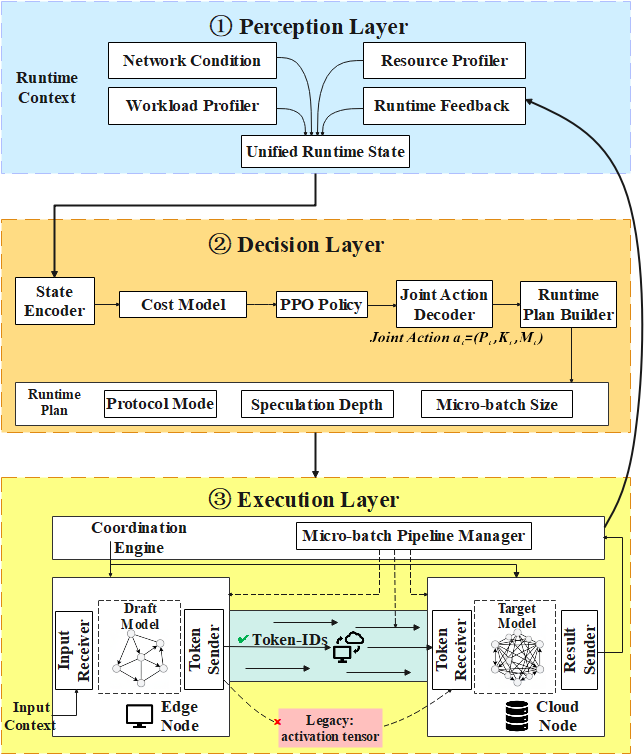
\includegraphics[width=\linewidth,height=\textheight,keepaspectratio]{fig6_framework.png}
    \caption{Overall architecture of DeepFlow RL.}
    \label{fig:6}
\end{figure}

At each decision step, the system first constructs a runtime observation and maps it to a unified decision vector $a_t$. Once an action is issued, the unified execution backend instantiates it into an executable plan under the same physical assumptions, feasibility checks, and stage-timing logic, and returns feedback signals such as throughput, makespan, bottleneck labels, and memory feasibility. These feedback signals are then fed into the next round of state construction, allowing training and evaluation to share the same closed-loop execution semantics.

\paragraph{Perception Layer.}
The perception layer is responsible for collecting and organizing the runtime context required for adaptive scheduling. In the current implementation, the observed system state is defined as
\begin{equation}
s_t = (W_t, \tau_t, L_t, T_{t-1}),
\end{equation}
As illustrated in Fig.~\ref{fig:6}, these runtime signals are aggregated into a unified state via online profiling and feedback collection. This unified representation enables the controller to both react to changing network conditions and adapt based on recent execution outcomes. Furthermore, the state design is extensible: finer-grained control can be supported by incorporating additional signals, such as memory utilization, device load, prefix reuse statistics, or historical micro-batch behavior.

\paragraph{Decision Layer.}
The decision layer is deployed on the edge side and serves as the central controller of DeepFlow RL. Given the runtime state $s_t$, it performs state encoding and cost-aware decision making, and outputs the corresponding joint decision over protocol mode, speculative depth, and micro-batch granularity. As shown in Fig.~\ref{fig:6}, this layer transforms the unified runtime state into an executable runtime plan through a policy-guided action generation process. Its state space, action space, and reward function will be further described in Section~5.4.

\paragraph{Execution Layer.}
The execution layer is responsible for realizing the runtime plan generated by the decision layer. As shown in Fig.~\ref{fig:6}, it consists of a collaborative inference backend, including protocol execution, micro-batch pipeline management, and performance feedback generation. After receiving $a_t$, the execution layer first selects the corresponding transmission protocol according to $P_t$, then performs edge-side drafting and cloud-side verification according to $K_t$, and finally organizes the global request stream into multiple micro-batches according to $M_t$. This layer is built on top of a unified discrete-event execution backend, which ensures that the same physical assumptions, scheduling logic, and feasibility checks are used consistently in both policy training and offline evaluation. During execution, the backend tracks the interaction among drafting latency, communication latency, cloud verification cost, and memory constraints, and returns the resulting throughput, makespan, bottleneck category, and feasibility outcome to the controller. 

\subsection{Distributed Token-Based Speculative Inference Protocol}

The core mechanism of DeepFlow RL is a distributed token-based speculative inference protocol, illustrated in Fig.~\ref{fig:7}. Its basic verification logic still follows the draft-verify principle of speculative decoding: a lightweight draft model first proposes candidate tokens, and a stronger target model then verifies them in parallel \cite{leviathan2023speculative,li2024eagle,miao2024specinfer}. However, unlike conventional speculative decoding in single-node or tightly coupled serving frameworks, our approach does not simply transplant this mechanism into the edge-cloud setting. Instead, it repurposes the draft--verify structure as a semantic-level cross-device transmission protocol. In this framework, speculative inference no longer serves only as a local decoding accelerator, but also acts as the transmission primitive for weak network edge-cloud collaboration: the system uses compact token-ID payloads to replace high-dimensional activation transfer, thereby shifting collaborative overhead from activation-heavy communication to lightweight semantic-level exchange.

\begin{figure*}[t]
    \centering
    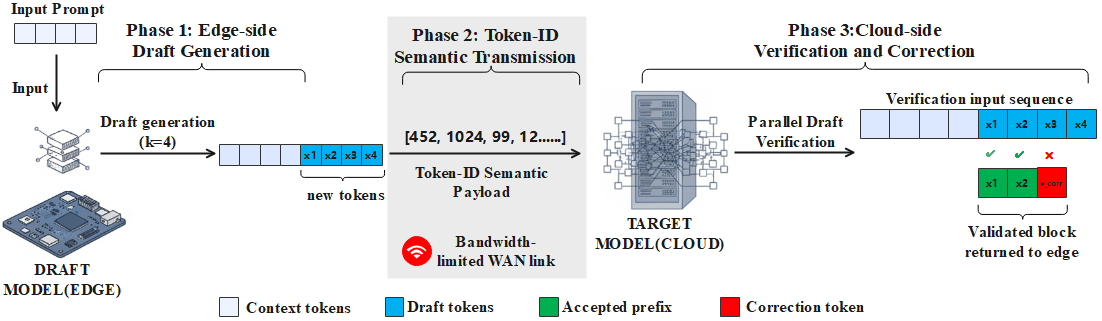
\includegraphics[width=0.96\textwidth]{fig7_core.png}
    \caption{Core mechanism of token-based speculative collaboration.}
    \label{fig:7}
\end{figure*}

\begin{algorithm}[t]
\caption{Distributed Token-Based Speculative Inference}
\label{alg:token_spec_protocol}
\begin{algorithmic}[1]
\Require Context $X$, draft model $\mathcal{M}_d$ on edge, target model $\mathcal{M}_{\mathrm{tar}}$ on cloud, action $(P,K,M)$
\Ensure Validated outputs for all micro-batches

\State Split the global batch into micro-batches of size $M$
\For{each micro-batch $b_i$}
    \State \textbf{Edge drafting:} generate $K$ candidate tokens
    \[
    \mathcal{B}^{(i)}_{\mathrm{draft}}=\{x^{(i)}_1,\ldots,x^{(i)}_K\}
    \]
    \If{$P = 0$}
        \State Serialize and transmit token IDs of $\mathcal{B}^{(i)}_{\mathrm{draft}}$
    \Else
        \State Execute target-model prefix layers $1,\ldots,P$ on edge
        \State Serialize and transmit the activation tensor at split point $P$
    \EndIf
    \State \textbf{Cloud verification:} run one parallel verification pass with $\mathcal{M}_{\mathrm{tar}}$
    \State Find the first mismatch position and accept the matched draft prefix
    \State Generate one correction token $x^{(i)}_{\mathrm{corr}}$
    \State Return the validated block
    \[
    \Delta X^{(i)}=\{x^{(i)}_1,\ldots,x^{(i)}_n,x^{(i)}_{\mathrm{corr}}\}
    \]
    \State Synchronize $\Delta X^{(i)}$ back to the edge context
\EndFor
\State \Return $\{\Delta X^{(i)}\}_{i=1}^{N}$
\end{algorithmic}
\end{algorithm}

For an input context $X_t$, the protocol proceeds through the following three phases.

\paragraph{Phase 1: Edge-side Draft Generation.}
The edge device runs the draft model $\mathcal{M}_d$ to generate $K$ candidate tokens in an autoregressive manner:
\begin{equation}
x_j = \arg\max_v p_{\mathcal{M}_d}(v \mid X_t, x_{1:j-1}), \quad j\in\mathcal{J}.
\end{equation}

The resulting draft block is denoted as
\begin{equation}
B_{\mathrm{draft}} = \{x_1, \ldots, x_K\}.
\end{equation}
This phase remains on the edge side because a smaller draft model can generate candidate continuations with relatively low latency, without invoking the full cloud model for every token. As shown in Fig.~\ref{fig:7}, the edge acts as a fast local proposer that produces a speculative token block before any cross-device synchronization is triggered.

\paragraph{Phase 2: Token-ID Semantic Transmission.}
After the draft block is generated, the edge transmits a compact semantic payload to the cloud. When the protocol operates in DeepFlow mode ($P=0$), the transmitted payload consists only of token IDs rather than intermediate activations. As defined in Section~4, the corresponding communication volume scales linearly with the micro-batch size and speculative depth, because each transmitted token ID is encoded as a 32-bit integer. The key point here is the change of the cross-device transmission primitive itself: DeepFlow RL rewrites the transmission primitive as a semantic-level token-ID payload, thereby making collaborative inference under weak network conditions systemically feasible in a different way.

\paragraph{Phase 3: Cloud-side Verification and Correction.}
After receiving the transmitted draft block, the cloud-side target model $\mathcal{M}_t$ performs parallel verification conditioned on the current context. Instead of verifying candidate tokens one by one through sequential edge-cloud interaction, the target model evaluates the whole draft block in parallel and determines the longest accepted prefix:
\begin{equation}
r = \max \left\{ j\middle|\, x_i = y_i,\ \forall i \le j ,j \in\mathcal{J} \right\}
\end{equation}
where $y_i$ denotes the token preferred by the target model at position $i$. The cloud then immediately generates one correction token after the accepted prefix:
\begin{equation}
x_{\mathrm{corr}} \sim p_{\mathcal{M}_t}\bigl(\cdot \mid X_t, x_{1:r}\bigr).
\end{equation}
Accordingly, the validated output block returned by the cloud is
\begin{equation}
\Delta X = \{x_1, \ldots, x_r, x_{\mathrm{corr}}\}.
\end{equation}

This validated block is then synchronized back to the edge, as shown in Fig.~\ref{fig:7}. The cloud does not need to return the entire historical context; it only returns the newly validated increment, namely the accepted draft prefix and one correction token. The edge appends $\Delta X$ to its local context and starts the next speculative round. In general, draft tokens have a non-zero acceptance probability, so the number of effective output tokens produced in one collaborative round is greater than one; this is the fundamental reason why speculative collaboration can improve end-to-end throughput. The specific optimal speculative depth, however, depends on the system-level trade-off among acceptance gain, draft generation cost, cloud verification cost, and resource overhead. The overall protocol is summarized in Algorithm~\ref{alg:token_spec_protocol}.

\subsection{Phase-Aware micro-batch Pipeline Scheduler}

Although token-ID transfer substantially reduces communication volume, significant temporal asymmetry remains among edge drafting, network transmission, and cloud verification. Consequently, purely sequential execution incurs stop-and-wait inefficiency and underutilizes the cloud. To address this, we adopt a phase-aware micro-batch pipeline scheduler that partitions the global batch by micro-batch size and pipelines execution across three stages: edge computation, network transmission, and cloud verification. The scheduler maintains the availability pointers of different stages in a discrete-event manner, as summarized in Algorithm~\ref{alg:pipeline_scheduler}.

\begin{algorithm}[!htbp]
\caption{Phase-Aware micro-batch Pipeline Scheduling}
\label{alg:pipeline_scheduler}
\begin{algorithmic}[1]
\Require Total batch size $B$, micro-batch size $M$, action $(P,K,M)$, runtime state $s_t$
\Ensure Makespan $T_{\mathrm{make}}$, throughput $\mathcal{T}$, timeline $\Gamma$

\State $N \gets \lceil B/M \rceil$
\State Initialize availability pointers:
\[
t_e \gets 0,\quad t_n \gets 0,\quad t_c \gets 0
\]
\State $\Gamma \gets \emptyset$

\For{$i = 1$ to $N$}
    \State Compute stage durations for micro-batch $i$:
    \[
    T_e^{(i)},\; T_n^{(i)},\; T_c^{(i)}
    \]
    \State $s_e^{(i)} \gets t_e$
    \State $e_e^{(i)} \gets s_e^{(i)} + T_e^{(i)}$
    \State $t_e \gets e_e^{(i)}$

    \State $s_n^{(i)} \gets \max(e_e^{(i)}, t_n)$
    \State $e_n^{(i)} \gets s_n^{(i)} + T_n^{(i)}$
    \State $t_n \gets e_n^{(i)}$

    \State $s_c^{(i)} \gets \max(e_n^{(i)}, t_c)$
    \State $e_c^{(i)} \gets s_c^{(i)} + T_c^{(i)}$
    \State $t_c \gets e_c^{(i)}$

    \State Append stage records of micro-batch $i$ to timeline $\Gamma$
\EndFor

\State $T_{\mathrm{make}} \gets t_c$
\State $N_{\mathrm{eff}} \gets B \cdot \mathbb{E}[Y(K)]$
\State $\mathcal{T} \gets N_{\mathrm{eff}} / T_{\mathrm{make}}$
\State \Return $(T_{\mathrm{make}}, \mathcal{T})$
\end{algorithmic}
\end{algorithm}

Given the total batch size $B$ and the micro-batch size $M$, the scheduler first partitions the batch into
%\begin{equation}
$N = \left\lceil \frac{B}{M} \right\rceil$
%\end{equation}
micro-batches, and models execution as a three-stage pipeline consisting of edge computation, network transmission, and cloud verification. For micro-batch $i$, the stage start and end times satisfy the following discrete-event progression:
\begin{align}
s_e^{(i)} &= e_e^{(i-1)}, &
e_e^{(i)} &= s_e^{(i)} + T_e^{(i)}, \\
s_n^{(i)} &= \max\!\left(e_e^{(i)}, e_n^{(i-1)}\right), &
e_n^{(i)} &= s_n^{(i)} + T_n^{(i)}, \\
s_c^{(i)} &= \max\!\left(e_n^{(i)}, e_c^{(i-1)}\right), &
e_c^{(i)} &= s_c^{(i)} + T_c^{(i)}.
\end{align}
The final makespan is
\begin{equation}
T_{\text{make}} = e_c^{(N)}.
\end{equation}

micro-batch pipelining is not a monotonically beneficial mechanism: when strong stage asymmetry exists, both overly coarse and overly fine granularity may lead to suboptimal system behavior \cite{zhong2024distserve,hu2025bestserve}. Larger micro-batches reduce the number of stage switches, but may weaken cross-stage overlap opportunities; smaller micro-batches are more favorable for filling the pipeline, but may also amplify RTT-driven stop-and-wait and handshake overhead. Therefore, micro-batch granularity itself is a system-level trade-off variable rather than a fixed hyperparameter.

\subsection{PPO-Based Adaptive Controller}

To adaptively select $(P,K,M)$ under dynamic network and workload conditions, DeepFlow RL formulates the scheduling problem as a Markov decision process and adopts proximal policy optimization (PPO) as the controller \cite{schulman2017ppo}. At decision step $t$, the DRL scheduler takes as input the runtime state defined in Section~4 and outputs a discrete joint action over protocol mode, speculative depth, and micro-batch granularity. 

Given state $s_t$ and action $a_t$, the unified backend returns throughput, feasibility, and memory statistics. The reward is defined as
\begin{equation}
r_t=
\begin{cases}
\log\!\big(T(a_t;s_t)+\varepsilon\big), & a_t \in \mathcal{F}(s_t),\\
-\lambda_{\text{oom}}-\lambda_{\text{pen}}\Delta_{\text{mem}}, & a_t \notin \mathcal{F}(s_t),
\end{cases}
\end{equation}
where $T(a_t;s_t)$ denotes the effective throughput computed by the backend, $\Delta_{\text{mem}}$ denotes the relative memory-budget violation, and $\lambda_{\text{oom}},\lambda_{\text{pen}}>0$ are infeasibility penalty terms. This design encourages the agent to maximize throughput while avoiding OOM actions. The reward uses the logarithm of effective throughput to reduce training instability caused by large return-scale differences across scenarios, and to make the controller focus more on relative performance improvement under feasible conditions.

Let $\theta$ denote the policy parameters. PPO optimizes the following clipped surrogate objective \cite{schulman2017ppo}:
\begin{equation}
L^{\mathrm{PPO}}(\theta)=
\mathbb{E}_t\left[
\min\left(
r_t(\theta)\hat{A}_t,\,
\mathrm{clip}(r_t(\theta),1-\epsilon,1+\epsilon)\hat{A}_t
\right)
\right].
\end{equation}

During training, the controller interacts with the unified backend under randomized scenarios of bandwidth, latency, and prompt length; during deployment, the perception layer collects runtime signals, the policy outputs $(P,K,M)$, and the execution layer carries out the corresponding plan. Reinforcement learning thus serves as a runtime controller over the unified feasible region, learning the mapping from system states to joint actions.

\subsection{End-to-End Training and Inference Workflow}

\begin{algorithm}[t]
\caption{PPO-Based Adaptive Scheduling in DeepFlow RL}
\label{alg:ppo_training}
\begin{algorithmic}[1]
\Require Policy $\pi_\theta$, value network $V_\phi$, unified simulator backend $\mathcal{E}$, training distribution $\mathcal{D}$
\Ensure Trained policy $\pi_{\theta^\star}$

\For{each training episode}
    \State Sample a scenario from domain randomization:
    \[
    (W_t,\tau_t,L_t)\sim \mathcal{D}
    \]
    \State Construct observation
    \[
    s_t=(W_t,\tau_t,L_t,\mathcal{T}_{t-1})
    \]
    \State Sample action
    \[
    a_t=(P_t,K_t,M_t)\sim \pi_\theta(\cdot|s_t)
    \]
    \State Execute $a_t$ in the unified backend $\mathcal{E}$
    \State Obtain:
    \[
    \mathcal{T}(a_t;s_t),\; \text{feasible},\; \text{memory ratios},\; \text{bottleneck}
    \]
    \State Compute reward
    \[
    r_t=
    \begin{cases}
    \log(\mathcal{T}(a_t;s_t)+\varepsilon), & \text{if feasible}\\
    -\lambda_{\mathrm{oom}}-\lambda_{\mathrm{pen}}\Delta_{\mathrm{mem}}, & \text{otherwise}
    \end{cases}
    \]
    \State Store transition $(s_t,a_t,r_t,s_{t+1})$
    \State Estimate advantages $\hat{A}_t$ and returns
    \State Update $(\theta,\phi)$ using PPO clipped objective
\EndFor
\State \Return $\pi_{\theta^\star}$
\end{algorithmic}
\end{algorithm}

The end-to-end workflow of DeepFlow RL integrates both the offline training stage and the online inference stage, as shown in Algorithm~\ref{alg:ppo_training}. During training, the agent continuously interacts with the unified analytical backend under diverse scenarios through domain randomization. In each episode, the environment randomly initializes the network bandwidth $W_t$, round-trip latency $\tau_t$, and prompt length $L_t$, thereby constructing the state observation $s_t$. The PPO agent then outputs the joint action $a_t$, which is executed by the unified backend. The environment computes the reward and updates the PPO policy parameters according to the returned performance metrics, namely effective throughput and memory feasibility status.

During online inference, the system operates in a tightly coupled closed loop. The perception layer first dynamically collects real-time bandwidth, latency, and context length. These observations are then sent to the decision layer, where the pretrained PPO policy directly infers the joint action $(P,K,M)$. Based on this decision, the execution layer organizes one speculative collaborative inference step using the selected transmission protocol and micro-batch granularity. The validated tokens are then synchronized back to the edge to update the context, and this generation loop repeats until the whole sequence is completed.

This architecture establishes a continuous feedback loop. The perceived state determines the action; the action sets the protocol mode, speculative depth, and pipeline granularity; and the execution result drives the system into the next state. This enables DeepFlow RL to adapt its micro-batch strategy within the unified memory-feasible region based on dynamic RTT and workload characteristics.


\section{Experimental Evaluation}
\subsection{Experimental Setup}
%\subsubsection{Experimental Platform and Unified Simulator}

All experiments in this paper are conducted on a unified resource-aware analytical simulation backend. Under consistent execution semantics, this backend jointly models edge-side drafting, cross-device communication, cloud-side verification, micro-batch pipelining, and memory-feasibility constraints, while also supporting the training environment, standalone validation scripts, and experiment scripts. With this design, policy training, baseline comparison, and final evaluation share the same execution kernel, thereby avoiding bias introduced by inconsistencies between the training backend and the evaluation backend. This setting is consistent with the general practice of analytical performance modeling, discrete-event simulation, and LLM serving simulators: prior work usually emphasizes comparable modeling and analysis of system design, resource constraints, and execution behavior under unified assumptions, rather than reproducing every detail of a specific software stack or hardware microarchitecture. Therefore, the reported results should be understood as comparative systems conclusions under a consistent resource-constrained model, rather than absolute deployment-level performance predictions \cite{williams2009roofline,agrawal2024vidur,cho2025llmservingsim2,qin2026phantora}.

In our experiments, the edge side and the cloud side are configured with reference to NVIDIA Jetson AGX Orin 64GB and NVIDIA A100-PCIE-80GB respectively. We do not directly use the nominal peak specifications of these devices. Instead, we model them in the unified simulator using calibrated effective parameters that incorporate efficiency discounting, runtime reservation, and memory-budget constraints. Specifically, the effective compute throughput, effective memory bandwidth, and available memory budget on the edge are set to 24.70 TFLOPS, 115.20 GB/s, and 46.00 GB, respectively. The corresponding values on the cloud are 162.24 TFLOPS, 1321.75 GB/s, and 70.00 GB. The target model is Llama-2-7B with 32 layers. A lightweight draft model is deployed on the edge, while the target model is deployed on the cloud for verification and correction.

\subsubsection{Workloads and Network Scenarios}

To comprehensively evaluate the adaptability of DeepFlow RL under different edge-cloud collaborative settings, we construct experimental scenarios along two dimensions: workloads and network conditions.

On the workload side, we mainly examine the influence of different prompt lengths on inference behavior. The main configuration is
\begin{equation}
L \in \{128,\,512,\,2048,\,4096\}.
\end{equation}
Short prompts are used to examine granularity adjustment behavior in high-throughput regions, whereas medium and long prompts are used to study how verification cost, memory pressure, and bottleneck shifts affect system decisions.

On the network side, we separately examine the variation of bandwidth and latency. The bandwidth sweep is
\begin{equation}
W \in \{0.5,\,1,\,2,\,5,\,10,\,50,\,100\}\ \text{Mbps},
\end{equation}
which is mainly used to evaluate the difference in bandwidth sensitivity between conventional activation-based partitioning and token-ID-based speculative collaboration. The latency settings cover both low-latency and high-RTT cases, with the main configuration given by
\begin{equation}
\tau \in \{10,\,30,\,50,\,100,\,120\}\ \text{ms}.
\end{equation}
The joint variation of bandwidth and RTT is used to examine their different effects on system behavior: the former mainly shapes the tolerability of activation transfer, while the latter more directly affects the stop-and-wait cost and stage-overlap benefit in micro-batch pipelining.

\subsubsection{Baselines}

To fairly evaluate the proposed method, all baselines are implemented under the same unified simulator and the same memory-aware feasible region, so that the differences among methods reflect only the differences in their decision spaces, rather than inconsistent feasibility criteria or throughput definitions. For each method, we search only within its allowed action subspace and report the best feasible action within that subspace. We compare the following five types of baselines: i) \emph{Best Feasible Local Only}, which executes inference entirely on the edge device; ii) \emph{Best Feasible Cloud Only}, which relies entirely on cloud execution; iii)\emph{Best Feasible Legacy Split}, which represents conventional collaborative inference with activation transfer for $P>0$; iv) \emph{Best Static DeepFlow}, which denotes the best static configuration obtained by offline enumeration under DeepFlow mode; and v) \emph{Best PPO (Ours)}, which learns the mapping from states to actions through PPO and directly outputs actions during evaluation.

\subsubsection{PPO Training Configuration}

PPO serves as the adaptive controller and is trained in the unified environment. During training, actions are sampled from the policy distribution, while during evaluation, the final action is produced by deterministic policy inference. Both training and evaluation call the same memory-aware simulator and use the same reward semantics and infeasible-action penalty logic, thereby avoiding additional bias between the training objective and the final test semantics. During training, the environment samples different bandwidths, latencies, and prompt lengths through domain randomization, in order to improve the generalization ability of the policy across diverse scenarios. Both the policy network and the value network are implemented as two-layer multilayer perceptrons, with 256 hidden units in each layer. The state input is normalized to reduce training instability caused by heterogeneity in feature scales. This configuration follows the common use of PPO in systems-control tasks, where a relatively simple but stable function approximator is combined with environment randomization to learn a robust mapping from scenarios to actions \cite{schulman2017ppo,qin2026twostageppo}.

\subsubsection{Evaluation Metrics}

DeepFlow RL is evaluated from both performance and resource-aware perspectives. The primary metric is throughput, defined as the number of effective tokens produced per unit time, i.e., $N_{\mathrm{eff}} / T_{\mathrm{make}}$. We also report makespan to characterize the end-to-end batch completion time.

To analyze feasibility and resource pressure, we further measure the feasible ratio of the action space, the OOM distribution on the edge and the cloud, and the memory ratio, defined as the ratio between peak memory usage and the corresponding memory budget. Finally, to explain performance variation and policy quality, we record the dominant bottleneck type returned by the unified backend, and, when applicable, the oracle gap between the PPO policy and the feasible oracle. Taken together, these metrics allow us not only to compare different collaborative strategies, but also to reveal the underlying resource constraints, bottleneck shifts, and decision patterns.

%\subsection{Experimental Results and Analysis}
\subsection{Deepflow Performance}
%\subsubsection{Main Results}

A comparison is first made between DeepFlow RL and different feasible baselines under the unified memory-aware simulator. All methods are evaluated under the same execution semantics, feasible-region definition, and throughput metric. Therefore, the performance differences reflect only the differences in the action subspaces accessible to each method, rather than inconsistencies in backend implementation or constraint settings.

\paragraph{Overall comparison under weak network.}
Unlike the fixed-action illustrative comparison in Section 3.2, here we report the best feasible end-to-end baseline results under the unified evaluation setting. Fig.~\ref{fig:8} shows the overall comparison under a representative weak network scenario (1 Mbps, 50 ms, prompt length $=512$). \emph{Best Feasible Local Only} achieves only 3.59 tok/s, suggesting that under the current edge-device configuration, fully local execution is insufficient for efficient LLM inference. \emph{Best Feasible Cloud Only} improves throughput to 23.05 tok/s, indicating that moving the main computation to the cloud can indeed alleviate the compute bottleneck on the edge; however, its end-to-end efficiency is still limited by cross-device interaction overhead. In contrast, the conventional \emph{Best Feasible Legacy Split} reaches only 10.55 tok/s, which is significantly lower than cloud-only execution. This suggests that under weak network conditions, activation-based collaboration cannot fully realize the potential of edge-cloud inference, and instead introduces additional overhead through intermediate-state transmission.

\begin{figure}
    \centering
    \includegraphics[width=0.96\columnwidth]{fig8_overall_comparison.pdf}
    \caption{End-to-end throughput comparison under a representative weak network setting.}
    \label{fig:8}
\end{figure}

Under the same scenario, both \emph{Best Static DeepFlow} and \emph{Best PPO (Ours)} reach 39.53 tok/s, achieving an 11.01$\times$ throughput improvement over the best feasible local-only baseline, while also substantially outperforming cloud-only and legacy split. This result indicates that token-ID-based speculative collaboration can effectively reduce collaborative overhead under weak network conditions.

\paragraph{Cross-scenario comparison against the best static configuration.}

\begin{table*}[!t]
    \centering
    \caption{Cross-scenario comparison between the PPO policy and the best static DeepFlow configuration.}
    \label{tab:cross_scenario_generalization}
    \begin{tabular*}{0.85\textwidth}{@{\extracolsep{\fill}} l c c l @{}}
        \toprule
        \textbf{Scenario} & \textbf{Best Static DeepFlow} & \textbf{Best PPO} & \textbf{PPO Action} \\
        \midrule
        Weak Net / Short Prompt     & 39.53 & 39.53 & $P{=}0, K{=}1, \mathrm{MB}{=}2$ \\
        Moderate Net / Short Prompt & 41.23 & 41.23 & $P{=}0, K{=}1, \mathrm{MB}{=}1$ \\
        Strong Net / Short Prompt   & 41.82 & 41.82 & $P{=}0, K{=}1, \mathrm{MB}{=}1$ \\
        \addlinespace
        Weak Net / Long Prompt      & 10.05 & 10.05 & $P{=}0, K{=}1, \mathrm{MB}{=}1$ \\
        Strong Net / Long Prompt    & 10.12 & 10.12 & $P{=}0, K{=}1, \mathrm{MB}{=}1$ \\
        \bottomrule
    \end{tabular*}
\end{table*}

To further evaluate the behavior of the learned policy across scenarios, we compare PPO with \emph{Best Static DeepFlow} under representative settings. As shown in Table~\ref{tab:cross_scenario_generalization}, PPO recovers throughput that is identical or nearly identical to \emph{Best Static DeepFlow} across typical scenarios, including weak network/short prompt, moderate network/short prompt, strong network/short prompt, weak network/long prompt, and strong network/long prompt. This suggests that PPO does not simply memorize a fixed action for one particular operating point. Instead, it learns a state-to-action mapping that adjusts with workload and network conditions, and approaches high-quality solutions obtained by static enumeration over the unified feasible region.

\paragraph{Bandwidth sensitivity.}

\begin{figure}
    \centering
    \includegraphics[width=0.96\columnwidth]{fig9_bandwidth_sensitivity.pdf}
    \caption{Bandwidth sensitivity of different collaborative strategies.}
    \label{fig:9}
\end{figure}

A comparison is first made between DeepFlow RL and different feasible baselines under the unified memory-aware simulator. As shown in Fig.~\ref{fig:9}, under prompt length $=512$ and latency $=50$ ms, the throughput of \emph{Best Feasible Legacy Split} increases from 5.85 tok/s at 0.5 Mbps to 24.78 tok/s at 100 Mbps, showing clear bandwidth dependence. This indicates that conventional activation-based partitioning is highly constrained by link capacity, and that its dominant bottleneck comes from cross-device transmission of high-dimensional intermediate states. In contrast, \emph{Best Static DeepFlow} and \emph{Best PPO} remain almost unchanged across the whole bandwidth sweep, with throughput staying around 39.52--39.53 tok/s. This result suggests that token-ID transfer compresses the communication payload to a level at which the system is no longer primarily bandwidth-dominated within the examined range.

\subsection{Policy Behavior Analysis}

\begin{figure*}[t]
    \centering
    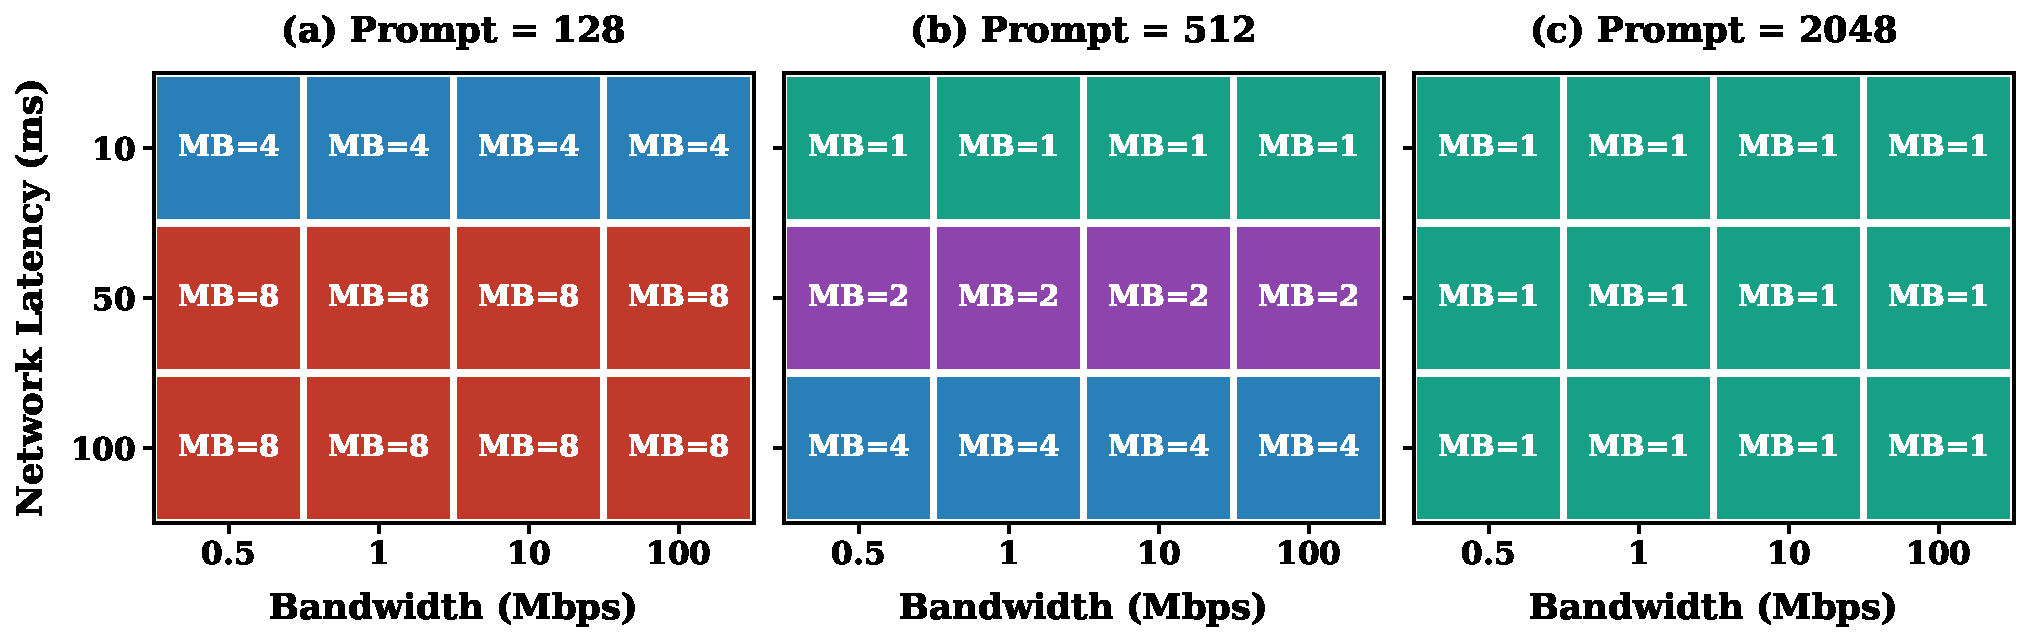
\includegraphics[width=0.96\textwidth]{fig10_combined_policy_map.pdf}
    \caption{Learned policy map across bandwidth, latency, and prompt length.}
    \label{fig:10}
\end{figure*}

The main results show that DeepFlow RL achieves stable performance gains under the unified memory-aware backend. This subsection further investigates the structure of the learned policy. Overall, the PPO policy does not form an irregular high-dimensional black-box action table. Instead, it exhibits a clear structural regularity: under representative scenarios, the policy consistently favors the token-ID collaborative mode with $P=0$ and tends to select shallow speculation with $K=1$, while the main degree of freedom that changes across scenarios is the micro-batch granularity $MB$.

As shown in Fig.~\ref{fig:10}, for shorter prompts, the policy selects larger micro-batches under higher RTT in order to amortize fixed round-trip cost. As prompt length increases, however, verification cost and memory pressure gradually become dominant, and the policy shifts toward smaller micro-batches, sometimes converging to $MB=1$. Therefore, what DeepFlow RL learns is not a simple fixed batching rule, but a structured policy built around \emph{stable protocol selection + adaptive granularity adjustment}.

\subsection{Feasibility and resource-aware Analysis}

Beyond throughput comparison, we also examine how memory budgets affect the optimal action in edge-cloud collaborative LLM inference. This section analyzes the resource-aware behavior of DeepFlow RL from five complementary perspectives: memory headroom, bottleneck shift, feasible-region shrinkage, OOM composition, and prompt-length-dependent throughput degradation.

\paragraph{Memory headroom of the learned policy.}

\begin{table}[t]
\centering
\caption{Memory headroom of the learned PPO policy under representative scenarios.}
\label{tab:mem_headroom}
\begin{tabular}{lcc}
\toprule
Scenario & Edge Peak / Budget & Cloud Peak / Budget \\
\midrule
\multicolumn{3}{c}{\textbf{Short Prompt Workloads}} \\
Weak      & 0.132 & 0.361 \\
Moderate  & 0.129 & 0.354 \\
Strong    & 0.129 & 0.354 \\
High RTT  & 0.137 & 0.377 \\
\midrule
\multicolumn{3}{c}{\textbf{Long Prompt Workloads}} \\
Weak      & 0.137 & 0.377 \\
Strong    & 0.137 & 0.377 \\
\midrule
\multicolumn{3}{c}{\textbf{Very Long Prompt Workloads}} \\
Weak      & 0.149 & 0.407 \\
Strong    & 0.149 & 0.407 \\
High RTT  & 0.149 & 0.407 \\
\bottomrule
\end{tabular}
\end{table}

If a high-performance strategy relies heavily on operating close to the memory limit, it often becomes less robust under workload variation. In contrast, DeepFlow RL selects high-yield actions while maintaining stable feasibility margins. Table~\ref{tab:mem_headroom} shows that the learned PPO policy remains feasible in all representative scenarios, with a clear safety margin from the OOM boundary. For short-prompt workloads, the edge-side memory ratio remains within [0.129, 0.137], while the cloud-side ratio stays within [0.354, 0.377]. As the prompt length increases to long and very long settings, both edge and cloud memory ratios increase systematically, with the edge-side ratio rising to 0.149 and the cloud-side ratio rising to 0.407. However, all values remain well below 1.

\paragraph{Action-space shrinkage under prompt-dependent memory constraints.}

\begin{figure}
    \centering
    \includegraphics[width=0.96\columnwidth]{fig11_feasible_ratio_vs_prompt.pdf}
    \caption{Action-space shrinkage under memory-aware constraints.}
    \label{fig:11}
\end{figure}

Next, how the feasible region of the joint action space changes with prompt length is examined. As shown in Fig.~\ref{fig:11}, as the prompt grows, edge-side draft KV, cloud-side verification KV, verification workspace, and related buffers all increase simultaneously. As a result, actions that are feasible under short contexts gradually leave the feasible action set because of memory constraints. This means that prompt length affects not only throughput, but also directly changes the structure of the feasible region faced by the scheduler. This is particularly important for a learning-based controller, which needs to learn not only \emph{which action yields higher benefit}, but also \emph{which actions are infeasible under the current resource condition}.

\paragraph{OOM composition across prompt lengths.}

\begin{figure}
    \centering
    \includegraphics[width=0.96\columnwidth]{fig12_oom_distribution.pdf}
    \caption{OOM composition under different prompt lengths.}
    \label{fig:12}
\end{figure}

In addition to feasible-region shrinkage, we further examine the OOM composition of infeasible actions. Fig.~\ref{fig:12} shows the OOM composition across different prompt lengths. Overall, under short prompts, infeasible actions are more likely to be triggered by the edge side, because larger micro-batches and deeper speculation first increase the memory pressure of the draft side and the prefix side. As the prompt continues to grow, the cloud-side verification workspace and suffix KV usage gradually become more dominant, making \emph{cloud} or \emph{both} types of OOM more common. This suggests that in the current edge-cloud setting, the memory bottleneck is not statically fixed on one side, but jointly shifts with workload scale and action choice.

\paragraph{Prompt length as the dominant resource factor.}

\begin{figure}
    \centering
    \includegraphics[width=0.96\columnwidth]{fig13_throughput_vs_prompt.pdf}
    \caption{Throughput degradation and bottleneck convergence under different prompt lengths.}
    \label{fig:13}
\end{figure}

Finally, we examine how throughput changes with prompt length. As shown in Fig.~\ref{fig:13}, even under token-ID collaborative mode, system throughput still gradually decreases as prompt length increases, because longer contexts simultaneously increase the sequence length of edge-side drafting, cloud-side verification cost, and memory pressure. This indicates that token-ID transfer does not remove the growth of verification and cache overhead inherent to LLM inference under long contexts. Once token-ID transfer suppresses the dominant communication bottleneck, prompt length becomes the main factor shaping verification cost, feasible-region shrinkage, and the bottleneck shift from the edge side toward the cloud side.

\section{Conclusion}

This paper studies edge-cloud collaborative large language model inference under weak network conditions. Unlike conventional collaborative inference, we repurpose speculative inference from a single-node decoding acceleration technique into a semantic-level transmission mechanism for edge-cloud collaboration. On this basis, we propose DeepFlow RL, a token-based speculative inference framework for adaptive edge-cloud collaborative LLM serving. With token-based speculative collaboration as its core, the framework uses micro-batch pipelining to mitigate stop-and-wait overhead under high-RTT settings, and further adopts PPO to learn the joint control of protocol mode, speculative depth, and micro-batch granularity. To ensure consistency between modeling and evaluation, we build a unified resource-aware analytical/discrete-event simulator that jointly models computation, communication, verification, memory feasibility, and system constraints. Experimental results on the unified backend show that DeepFlow RL substantially outperforms conventional activation-transfer-based collaborative baselines under representative weak network settings, while also exhibiting stable and interpretable policy behavior.

This work does not merely reuse speculative decoding as a single-node accelerator. Instead, it repurposes the draft–verify structure into an edge-cloud collaborative transmission primitive. Our results further demonstrate that, under weak network conditions, transforming the transmitted object provides greater systemic benefit than optimizing the partition boundary.


% -------------------------------------------------
% References
% -------------------------------------------------
\bibliographystyle{unsrtnat}
\bibliography{references}

\end{document}